\def\QRCODE{TB_IPR_TUT.IMG.boolean_models_pythonqrcode.png}
\def\QRPAGE{http://www.iptutorials.science/tree/master/TB_IPR/TUT.IMG.boolean_models/python}
\pcorrectionsection{Python correction}

%\begin{mcomment}
%\begin{mremark}
%Please notice that when using boolean arrays in python, the notations $1-X$ and $\sim X$ are equivalent. When using uint8 arrays, verify that the values range into [0;1].
%\end{mremark}
%\end{mcomment}
\begin{python}
import numpy as np
from skimage import draw
from scipy import misc,signal
import matplotlib.pyplot as plt
import progressbar
\end{python}

\subsection{Simulation of a 2-D Boolean model}
The process for simulating the proposed Boolean model of 2-D disks consists in four steps:
\begin{enumerate}
\item Generate the random number of points (by using the intensity parameter of the Poisson distribution). \\
In order to avoid edge effects, one consider a larger window than the observation window to generate the disks.
Indeed, a germ outside the observation window can generate a disk that intersects the observation window. 
\item Generate the random locations of the germs (random coordinates from a uniform distribution).
\item Generate the random size of the disks (random radius from a probability distribution).
\item Generate the union of disks.
\end{enumerate}
\vspace*{-8pt}
\begin{figure}[htbp]
\centering\caption{Boolean model of disks, with $Wsize=[1000,1000]$ and $RadiusParam=[10,30]$.}%
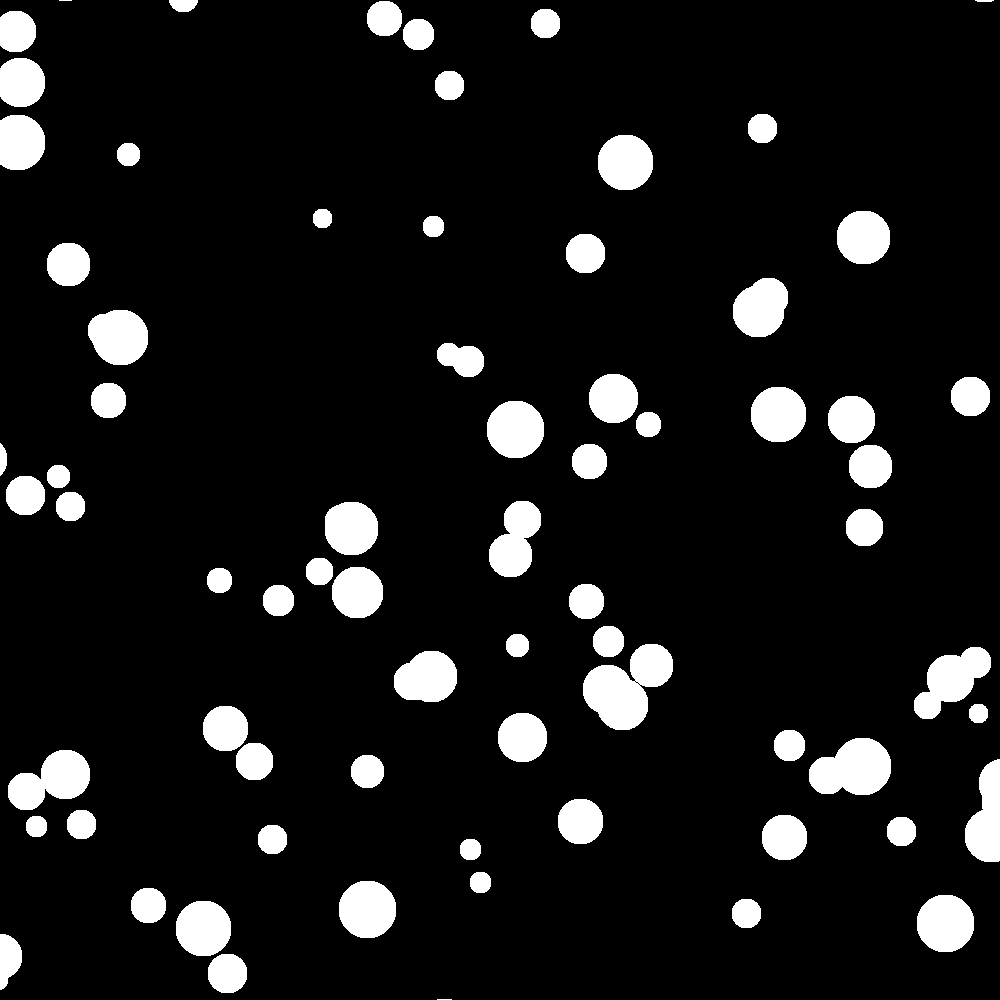
\includegraphics[width=.4\linewidth]{boolean_model.python.png}%
\label{fig:boolean_models:python:bmdisks}%
\end{figure}
\vspace*{-8pt}

When executing this simulation with the following parameters, we get a realization of the Boolean model as a binary image in Fig.\ref{fig:boolean_models:python:bmdisks}.

\begin{python}
Wsize=[1000, 1000]; 
gamma = 100 / (Wsize[0] * Wsize[1]);
radius = [10, 30];
Z = booleanModel(Wsize, gamma, radius);
plt.imshow(Z);
plt.show();
\end{python}


Here is the global function for generating such a Boolean model as a binary image:
\begin{python}
def booleanModel(Wsize, gamma, radius):
    """
    Generation of a 2D boolean model of disks, in a window of size Wsize
    Wsize: 2x1 array
    gamma: numerical value to control the Poisson process
    radius: min and max values of radii, 2x1 array
    returns: boolean array of size Wsize
    """
    edgeEffect =2 * np.max(radius) + 100;
    WsizeExtended = Wsize + 2*edgeEffect;
    # nb of points
    areaW = WsizeExtended[0] * WsizeExtended[1];
    nbPoints = np.random.poisson(lam = gamma * areaW);
    # positions of the germs
    x = np.random.randint(0, WsizeExtended[0], nbPoints);
    y = np.random.randint(0, WsizeExtended[1], nbPoints);
    # grains
    rGrains = np.random.randint(radius[0], radius[1], nbPoints);
    # union of grains
    Z = np.zeros((WsizeExtended[0], WsizeExtended[1]));
    for r, xx, yy in zip(rGrains, x, y):
        rr, cc = draw.circle(xx, yy, radius=r, shape=Z.shape)
        Z[rr, cc] = 1;
    # restrain window for side effects
    Z = Z[edgeEffect:edgeEffect+Wsize[0], edgeEffect:edgeEffect+Wsize[1]];
    return Z;
\end{python}



\subsection{Geometrical characterization of a 2-D Boolean model}
We can use the following function to compute the Minkowski functionals of the Boolean model (see the tutorial on Integral Geometry). The \pinline{regionprops} function from \pinline{skimage.measure} is not used because it computes the properties of each object.

\begin{python}
def minkowskiFunctionals(X):
    """
    Evaluation of the Minkowski functionals
    X: boolean 2D array
    returns area, perimeter, euler number N8, euler number n4
    
    """
    F = np.array([[0, 0, 0], [0, 1, 4], [0, 2, 8]]);
    XF = signal.convolve2d(X,F,mode='same');
    edges = np.arange(0, 17 ,1);
    h,edges = np.histogram(XF[:],bins=edges);
    f_intra = [0,1,0,1,0,1,0,1,0,1,0,1,0,1,0,1];
    e_intra = [0,2,1,2,1,2,2,2,0,2,1,2,1,2,2,2];
    v_intra = [0,1,1,1,1,1,1,1,1,1,1,1,1,1,1,1];
    EulerNb8 = np.sum(h*v_intra - h*e_intra + h*f_intra)
    f_inter = [0,0,0,0,0,0,0,0,0,0,0,0,0,0,0,1];
    e_inter = [0,0,0,1,0,1,0,2,0,0,0,1,0,1,0,2];
    v_inter = [0,1,0,1,0,1,0,1,0,1,0,1,0,1,0,1];
    EulerNb4 = np.sum(h*v_inter - h*e_inter + h*f_inter)
    Area = sum(h*f_intra)
    Perimeter = sum(-4*h*f_intra + 2*h*e_intra);
    
    return Area, Perimeter, EulerNb8, EulerNb4;

\end{python}

So we can estimate the Minkowski densites on different realizations of  the Boolean model:
\begin{python}
def realizations(Wsize, gamma, radius, n=100):
    """
    This function iterates the different realizations
    Wsize: window size
    gamma: value of gamma, see booleanModel
    radius: min and max values of the radii of the generated disks
    """
    W = np.zeros((n, 3));
    areaWsize = Wsize[0] * Wsize[1];
    bar = progressbar.ProgressBar();
    for i in bar(range(n)):
        Z = booleanModel(Wsize, gamma, radius);
        a, p, chi8, chi4 = minkowskiFunctionals(Z);
        W[i,:] = np.array([a, p/2, chi8*np.pi]) / areaWsize;
        
    return W;
\end{python}

Therefater, we can compare the estimated Minkowski mean densities of the Boolean model with the theoretical ones (by using the known parameters of the different probability distributions of this Boolean model):

\begin{python}
W = realizations(Wsize, gamma, radius, 1000);
W = np.mean(W, axis=0);
# comparison with analytical values
rMean = np.mean(radius);
areaMean = np.pi*rMean**2;
perMean = 2*np.pi*rMean;

W_X = gamma * np.array([areaMean, perMean/2, np.pi]);
W_0 = 1-np.exp(-W_X[0]);
W_1 = np.exp(-W_X[0]) * W_X[1];
W_2 = np.exp(-W_X[0]) * (W_X[2] - W_X[1]**2);

error_0 = np.abs(W_0-W[0]) / W_0;
error_1 = np.abs(W_1-W[1]) / W_1;
error_2 = np.abs(W_2-W[2]) / W_2;
\end{python}

\noindent Here are the results for 100 specific realizations:
\begin{sh}
errorW0:  0.0190201754056
errorW1:  0.200478931771
errorW2:  0.0342984925035
\end{sh}

The errors can be large due to the biais estimation of the Minkowski densities within an observation window (specifically for the perimeter and the Euler number). But you can use unbiased estimators which can be found in the literature.

\noindent Note that the Miles formulas can be inverted to estimate the Minkowski functionals of the typocal grain from the Minkowski mean densities of the Boolean model.
